\section{\textbf{Suspicious Text Detector}}
The key objective of our project is to design a system that can classify suspicious and non-suspicious text. \textbf{Fig} \ref{fig:proposed_model} shows an abstract view of our suspicious text detector classifier.

\begin{figure}[h!]
\centering
  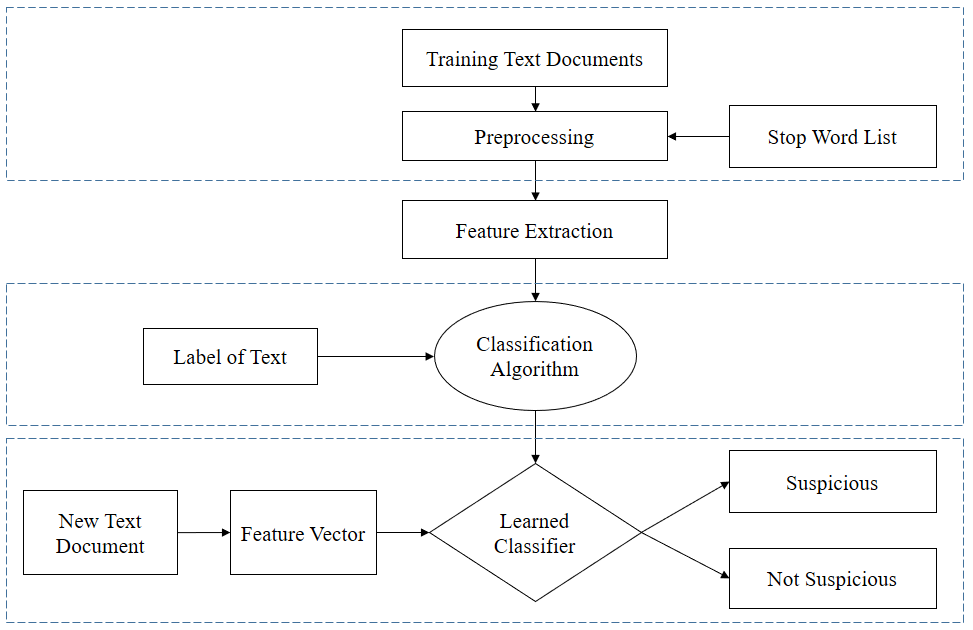
\includegraphics[height=6.8cm, width=8.8cm]{Figures/pr_model.PNG}
  \caption{ Model for Suspicious Text Detection}
  \label{fig:proposed_model}
\end{figure}

We have implemented this system by using different supervised machine learning algorithms. Our whole model is classified into four different phases.
\subsection{\textbf {Training Set Preparation}}
Our training set $T = \{t_1, t_2, t_3, ..., t_n\}$ is consist of $n$ training text documents. Each text is labeled as either suspicious or non suspicious. Suspicious class is denoted by $C_s$ and non suspicious class is denoted by $C_{ns}$.\par
A random text $t_i$ with $k$ words is represented by an one dimensional array $W[] =\{w_1, w_2, w_3, ....., w_k\}$ in our system,
\begin{table}[h!]
\begin{center}
\caption{Words of a Text}
\begin{tabular}{|m{1cm} | m{1cm}| m{1cm}|m{1cm} | m{1cm}|}
\hline
     $w_1$ & $w_2$  & $w_3$ & $...$ & $w_k$  \\
\hline
\end{tabular}
\end{center}
\end{table}

All texts are preprocessed by the preprocessor in order to remove inconsistencies for dataset. We have developed a list $S[]=\{s_1, s_2, s_3, ..., s_r\}$ with $r$ stopwords which is a column vector where each row contains a stop word.\par
\begin{table}[h!]
\begin{center}
\caption{Stop Word List}
\begin{tabular}{|m{0.7cm}|}
\hline
     $s_1$ \\
\hline
    $s_2$ \\
\hline 
    $s_3$ \\
\hline
 $...$ \\
 \hline
 $s_r$ \\
 \hline
\end{tabular}
\end{center}
\end{table}
\vspace{0.1cm}
In our system the word $w_i$ which has no contribution in deciding whether a text $t_i$ is suspicious ($C_s$) or not suspicious $(C_{ns})$ is referred as stop word $s_i$. Pronoun, conjunction, preposition, interjection, prefix and suffix are considered as stop words. Stop words $ s_1, s_2, s_3, ..., s_r$ are removed form the text $t_i$ by matching with a stop word list $S[]$. Punctuation's in a text are also removed in preprocessing step.


\subsection{\textbf{Feature Extraction}}
A word list is created by the tokenizer by tokenizing the main body of a text. Word frequencies is used as features in this system. Bag of words model is used to represent the features.
\renewcommand{\arraystretch}{1.3}
\begin{table}[h!]
\begin{center}
\caption{Feature Space}
\begin{tabular}{|m{0.7cm} | m{0.7cm}| m{0.7cm}|m{0.7cm} | m{0.7cm}|m{1cm}|m{0.7cm}|}
\hline
     & $w_1$ & $w_2$  & $w_3$ &$w_4$ &$...$ & $w_j$  \\
\hline
     $t_1$ & $2$ & $0$  & $0$ &$4$ &$...$ & $1$  \\
\hline
     $t_2$ & $0$ & $0$  & $1$ &$0$ &$...$ & $5$  \\
\hline
     $t_3$ & $4$ & $0$  & $2$ &$2$ &$...$ & $0$  \\
\hline
     $t_4$ & $0$ & $3$  & $0$ &$0$ &$...$ & $2$  \\
\hline
     $...$ & $...$ & ...  & $...$ &$...$ &$...$ & $...$  \\
\hline
     $t_i$ & $0$ & $0$  & $3$ &$1$ &$...$ & $0$  \\
\hline
\end{tabular}
\label{ff}
\end{center}
\end{table}
Table \ref{ff} shows the feature space for our system. Our feature space ($F[][]$) is a two dimensional ($i\times j$) array with $i$ rows and $j$ columns.
Here rows represents the texts $t_1, t_2, t_3, ..., t_i$ available in the corpus and columns represents total number unique words $w_1, w_2, w_3, ....., w_j$ in the corpus. Each cell of the array represents the frequency ($f_{ij}$) of a specific word $w_j$ occurs in a specific text $t_i$. Each row of the feature matrix represent features $F[][] =\{F[1], F[2], F[3], ... ,F[n]\} $ for the texts of the dataset. 

\subsection{\textbf{Classification Algorithm}}
It is most important part of our whole system. By using extracted features $F[1], F[2], F[3], ... ,F[n]$ and applying a suitable learning algorithm we train our model to classify texts as suspicious $C_s$ and non suspicious $C_{ns}$. Mainly logistic regression is used to implement the system and other algorithms are applied to establish comparison. 

\vspace{0.3cm}
\textbf{Naive Bayes}\cite{yoo2015classification} can be defined as Bayes theorem with a conditional independency assumption that all variables $A_{1},A_{2},...,A_{n}$ in a given category $C$ are conditionally independent with each other given $C$. 
According to Bayes rule for a text document $(T)$ and class $(C)$ we can write,
\begin{equation}
    P(C|T) = \frac{P(T|C)P(C)}{P(T)}
\end{equation}
Final equation for Naive Bayes classifier is,
\begin{equation}
     C_{MAP} = argmax P(X_{1},X_{2},...,X_{n}|C)P(C)
\end{equation}
\vspace{0.1cm}

\textbf{Logistic Regression}\cite{sharma2015active} is a binary classification model that predicts a binary outcome based on some features. The output of logistic regression depends on logistic function. The logistic function is a sigmoid function, which takes any real input and outputs a value between zero and one. The definition of logistic function or hypothesis function is,
\begin{equation}
    h_{\theta}(x) =  \frac{1}{1+\exp({-\theta^T x})}
\end{equation}
Cost function for Logistic regression is,
\begin{equation}
    J(\theta) = \frac{1}{m}\sum_{i-1}^{m}cost(h_{\theta}(x^{i}),y^{i})   
\end{equation}

\[
cost(h_{\theta}(x), y) = 
\begin{cases}
    -\log (h_{\theta}(x)) & \texttt{if } y = 1\\
     -\log (1-h_{\theta}(x)) & \texttt{if } y = 0
\end{cases}
\]
Here,\\
$m = $ Number of training examples.\\
$h_{\theta}(x^{i}) = $ Hypothesis function of $i_{th}$ training example\\
$y^i = $ Input label of $i_{th}$ training example.
\vspace{0.1cm}
\par
For binary logistic regression selecting
the threshold value is an important task, everything below threshold will considered as 0 or negative otherwise it will be 1 or positive.

\vspace{0.3cm}
\textbf{SVM}\cite{wei2012text} analyze data used for classification and regression analysis. SVM can perform linear classification as well as non-linear classification using kernel trick.

\vspace{0.3cm}
\textbf{KNN}\cite{harisinghaney2014text} is a non-parametric method used for
classification and regression. K nearest neighbors is a simple algorithm that stores all available cases and classifies new cases based on a similarity measure (e.g., distance functions).

\vspace{0.3cm}
A \textbf{Decision Tree}\cite{chavan2014survey} has two types of nodes one is external and another is internal. Decision classes are represented by external node of a decision tree. Internal nodes corresponds to attribute which are used for making decision by decision tree algorithm. Decision tree is simple to build and as it is a inductive algorithm it can be interpreted easily. Entropy is used to calculate the homogeneity of a sample.

\subsection{\textbf{Testing Phase}}
Testing is the most important phase for any machine learning model. Classification accuracy of the text classifier is calculated in testing phase. In our system testing phase is quite similar as training phase but in this part our learned classifier model is used for predicting. A test set $TS =\{ts_1, ts_2, ts_3, ..., ts_l\}$ is built to test the system which has $l$ text document. Sample texts are taken to test the system. After processing, using feature extraction methods features ($F[][]=\{F[1], F[2], F[3], ... ,F[l]\}$) are extracted from the testing texts $ts_1, ts_2, ts_3, ..., ts_l$. Our trained classifier model use this features to classify a text as suspicious ($C_s$) and non suspicious ($C_{ns}$).